\documentclass{article}
\usepackage[utf8]{inputenc}
\usepackage{setspace}
\usepackage{listings}
\usepackage{graphicx}
\usepackage[paper=portrait,pagesize]{typearea}
\usepackage{biblatex}
\usepackage[english]{babel} % To obtain English text with the blindtext package
\usepackage{blindtext}
\usepackage{csquotes}
\usepackage{multirow}
\usepackage{graphicx}
\usepackage[table,xcdraw]{xcolor}
\usepackage{float}

\addbibresource{references.bib}

\usepackage{xcolor}
\usepackage[colorlinks=true, allcolors=blue]{hyperref}
\usepackage[margin=1.2in]{geometry}


\definecolor{codegreen}{rgb}{0,0.6,0}
\definecolor{codegray}{rgb}{0.5,0.5,0.5}
\definecolor{codepurple}{rgb}{0.58,0,0.82}
\definecolor{backcolour}{rgb}{0.95,0.95,0.92}

\lstdefinestyle{mystyle}{
    backgroundcolor=\color{backcolour},   
    commentstyle=\color{codegreen},
    keywordstyle=\color{magenta},
    numberstyle=\tiny\color{codegray},
    stringstyle=\color{codepurple},
    basicstyle=\ttfamily\footnotesize,
    breakatwhitespace=false,         
    breaklines=true,                 
    captionpos=b,                    
    keepspaces=true,                 
    numbers=left,                    
    numbersep=5pt,                  
    showspaces=false,                
    showstringspaces=false,
    showtabs=false,                  
    tabsize=2
}
\lstset{style=mystyle}

\pagenumbering{gobble}
\title{MiniTwit Project \\DevOps, Software Evolution and Software Maintenance  \\
IT University of Copenhagen \\ Course code: BSDSESM1KU}
\date{1st of June 2022}
\author{ Group F \\
\begin{tabular}{l|l}
    \textbf{Name} & \textbf{E-mail} \\ \hline
    Jacob Møller Jensen & jacj@itu.dk      \\ \hline
    Marcus Sebastian Emil Holmgaard & seho@itu.dk \\ \hline
    Mikkel Møller Jensen & momj@itu.dk \\ \hline
    Rune Engelbrecht Henriksen & rhen@itu.dk \\ \hline
\end{tabular}
}

\begin{document}
\maketitle

\newpage
\tableofcontents
\newpage
\pagenumbering{arabic}
\section{System's perspective}
\subsection{Design}
When faced with the initial task of refactoring the MiniTwit system, we agreed to choose a stack consisting of technologies at least one member of the group had experience with.
This enabled us to both have the advantage of working with something familiar and gave the opportunity to learn something new. 

We chose React with Typescript for the frontend and when making the MiniTwit application we prioritized having the same functionality as the existing Flask application. As a result of this, the page setup and styling is identical to the original application.
We have used C\# for our backend. The data access technology used is Entity Framework Core.\\

Our Database is a Managed Azure SQL database hosted on Azure. Originally we had Azure SQL Edge running in Docker but as the database data is important to save persistently we switched to Azure SQL running on a Microsoft Azure server. Azure allowed us to enable automatic tuning of the different tables that improved performance drastically (Indexation of tables). More on these topics in future sections.

\subsection{Architecture}
This sections aims to describe the architecture of our system using Christensens 3+1 model \cite{architecturemodel} by showing:
\begin{itemize}
    \item Requirements
    \item Module viewpoint 
    \item Component \& connectors viewpoint 
    \item Allocation / deployment viewpoint
\end{itemize}

The system is separated into a three-tier architecture which is shown in Figure \ref{fig:Threetier}.
The diagram includes the course simulator (which is not in our control) as a component as it has a significant impact on the system.
\begin{figure}[H]
 \centering
 \includegraphics[width = 0.4\textwidth]{images/three\_tier.png}
 \caption{Overall architecture}
 \label{fig:Threetier}
\end{figure}

\subsubsection{Requirements}    
This section concerns the "+1" part of the 3+1 model i.e. the architectural requirements. \\
Though they referenced as "scenario-based" and "quality attribute-based" in the literature, this 
report will use the terms functional and non-functional requirements respectively. \\

\noindent
\textbf{Functional requirements}
\begin{enumerate}
    \item The system must provide the same functionality as the original MiniTwit system given at the introduction of the course
    \item The system must expose an API which adheres to the requirements of \cite{apispec} 
\end{enumerate} 

\noindent
\textbf{Non-functional requirements}
\begin{enumerate}
    \item The systems backend must be written in C\# 
    \item The systems frontend must be written in React with Typescript
    \item The system must be containerized with Docker ensuring isolation and portability
    \item The system must be deployed on DigitalOcean
    \item The system must be performant, scaleable and reliable in accordance to the SLA, Appendix \ref{app:SLA}.
\end{enumerate}
    
\subsubsection{Module viewpoint}
At the highest level, the system is divided into backend and frontend.\\

The following package diagram gives a high-level overview of the backend's file structure and dependencies.
\begin{figure}[H]
 \centering
 \includegraphics[width = 0.4\textwidth]{images/backend\_package\_overview.png}
 \caption{Backend Package overview showing how data is accessed in the system.}
 \label{fig:BackendPackageDiagram}
\end{figure}
\begin{itemize}
    \item \textbf{Domain:} contains the business entities of the system i.e. model and DTO classes representing users, tweets and followers.
    \item \textbf{DataAccess:} contains the class that handles sessions and communication with the database.
    \item \textbf{MiniTwitAPI:} houses the controller classes that make up both the public and internal APIs of the system, which are two separate units. 
\end{itemize}
A complete package diagram for the backend, including all relevant artifacts, etc., can be seen in figure \ref{fig:BackendCompletePackageDiagram}. \\

\begin{figure}[H]
 \centering
 \includegraphics[width = 0.5\textwidth]{images/backend\_complete\_package.png}
 \caption{Package diagram showing our backend artifacts, dependencies omitted for clarity}
 \label{fig:BackendCompletePackageDiagram}
\end{figure}

\newpage
The next part of the program is the frontend, of which a package diagram is shown in figure \ref{fig:FrontendPackageDiagram}.
Only the "src" package contains files of interest i.e. that we have written, as opposed to configuration or boilerplate files and as such the contents of "public", "nginx" and the root folder is not shown in the diagram. The artifacts represent the individual pages of the website as well as subcomponents, media, stylesheets and some configuration-files that are React-specific. The naming of the pages reflects the naming from the original page structure provided.

\begin{figure}[H]
 \centering
 \includegraphics[width = \textwidth]{images/package\_frontend.png}
 \caption{Package diagram of the frontend folder, some folders omitted for clarity}
 \label{fig:FrontendPackageDiagram}
\end{figure}


\subsubsection{Components \& connectors viewpoint}
Figure \ref{fig:CompleteComponentDiagram} shows the six components e.g. Docker containers of our primary DigitalOcean droplet and how they interact with each other at runtime. In the diagram, the "MiniTwit backend" component contains two separate API subcomponents. The actual Docker container uses the same port to handle both API requests from the simulator and from the website but we have chosen to show it as two components here to indicate that they serve two different purposes.
\begin{figure}[H]
 \centering
 \includegraphics[width = \textwidth]{images/all\_components.png}
 \caption{Component diagram of our primary DigitalOcean droplet, Docker volumes omitted}
 \label{fig:CompleteComponentDiagram}
\end{figure}
\subsubsection{Allocation / deployment viewpoint}
As seen in Figure \ref{fig:DeploymentDiagram}, the system consists of a managed database on Microsoft's Azure platform as well as two separate droplets on DigitalOcean. The two droplets constitute our scaling setup which is described in depth in a future section. \\
% The most interesting parts to examine more deeply (from an architectural perspective) is the Docker containers for frontend and backend, as we wrote the code for those parts whereas the remaining 4 Docker containers (on the minitwit droplet) are just third party dependencies. \\ 
\begin{figure}[H]
 \centering
 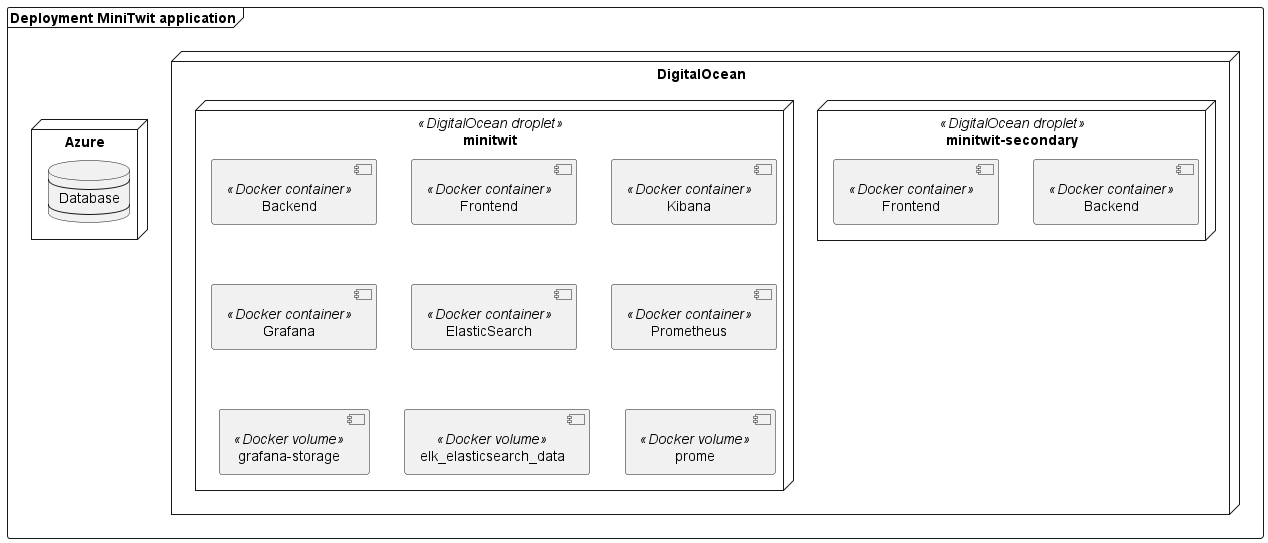
\includegraphics[width = \textwidth]{images/deployment.png}
 \caption{Deployment diagram illustrating the overall deployment view of our MiniTwit system including Docker volumes for monitoring and logging}
 \label{fig:DeploymentDiagram}
\end{figure}
\noindent
Both droplets are hosted on servers located in Frankfurt, Germany and have the following specs \\
\begin{table}[H]
\centering
\begin{tabular}{|l|l|l|l} 
\cline{1-3}
           & Primary & Secondary &   \\ 
\cline{1-3}
vCPU       & 1       & 1         &   \\ 
\cline{1-3}
Memory     & 2 GB    & 1 GB      &   \\ 
\cline{1-3}
Disc Space & 50 GB   & 25 GB     &   \\
\cline{1-3}
\end{tabular}
\end{table}

\noindent
They do not have the same specifications as they do not handle the same tasks but this will be elaborated in a later section.

\subsection{Dependencies - technologies and tools}
The following is a table of the dependencies and tools that the project relies on as well as a brief comment on what they're used for.
\centering
\begin{tabularx}{\textwidth}{|X|l|}
 \hline
 \textbf{Name} & \textbf{Responsibility}  \\ [0.5ex] 
 \hline\hline
 \textbf{Git} & Version control  \\ 
 \hline
 \textbf{GitHub} & Repository management \\
 \hline
 \textbf{C\# / ASP.NET CORE / .NET} & Used for our backend \\
 \hline
 \textbf{Typescript} & Used for React frontend \\
 \hline
 \textbf{Azure SQL Database} & The database system used for our MiniTwit application\\ 
 \hline
 \textbf{Serilog} & A library used for logging in the backend \\
 \hline
 \textbf{Prometheus} & Used for system monitoring \\
 \hline
 \textbf{Grafana} & Used to display monitoring information\\
 \hline
 \textbf{ElasticSearch} & Used to store the systems logs \\
 \hline
 \textbf{Kibana} & Used to present the aggregated logs \\
 \hline
 \textbf{Docker} & Used for containerizing the system \\
 \hline
 \textbf{Ubuntu} & The OS that our droplets run on\\
 \hline
 \textbf{React} & JavaScript library for building the website \\
 \hline
 \textbf{Nginx} & A web server that runs React\\
 \hline
 \textbf{Docker-compose} & Handling multiple docker containers \\
 \hline
 \textbf{Docker Hub} & Storing docker images \\
 \hline
 \textbf{Sonarcloud} & Static analysis \\
 \hline
 \textbf{DigitalOcean} & Provider of infrastructure \\
 \hline
 \textbf{Vagrant} & Provisioning of virtual machines \\
 \hline
 \textbf{CircleCI} & Continous integration pipeline \\
 \hline
 \textbf{Better Code Hub} & Provides static analysis of the code \\
 \hline
 \textbf{Keepalived} & High-availability / scaling \\
 \hline
 \textbf{Python} & Used in a script for switching floating IP on DigitalOcean  \\
 \hline
 \textbf{Bash} & Used as terminal for the developers and for scripts.\\
 \hline
 \textbf{SSMPT} & Used to configure the mail server.\\
 \hline
 \textbf{MailUtils} & Used to send a mail directly from a script using SSMTP server settings. \\
 \hline
 \textbf{Gmail} & Used as a central mailbox that forwards to our individual ITU mails \\[1ex] 
 \hline
\end{tabularx}

\subsection{Important interactions of subsystems}
The most important interactions of subsystems in our MiniTwit application are the following 
\begin{itemize}
    \item HTTP communication between frontend and backend
    \item HTTP communication between backend and the simulator
    \item HTTP communication between backend and Prometheus
    \item HTTP communication between Prometheus and Grafana
    \item HTTP communication between backend and ElasticSearch
    \item HTTP communication between ElasticSearch and Kibana
    \item Communication between the backend and the Azure database via EF Core
\end{itemize}

The sequence diagram in figure \ref{fig:SequenceDiagramPostMessage} shows the interaction between frontend, backend and database when a user posts a new message. \\
Most interactions between frontend and backend as well as between the backend and simulator follow the same flow, and as such these will not be depicted.

\begin{figure}[H]
 \centering
 \includegraphics[width = .5 \textwidth]{images/frontend\_backend\_post\_messages\_sequence.png}
 \caption{Sequence diagram depicting the interaction between frontend, backend and database when a user posts a new message}
 \label{fig:SequenceDiagramPostMessage}
\end{figure}

Figure \ref{fig:SequenceDiagramElasticBackendSim} shows an example of an interaction between the simulator, backend, ElasticSearch and database. In particular it depicts the sequence of logging and database calls that occur between a request to post a message being made and the response being returned to the simulator.

\begin{figure}[H]
 \centering
 \includegraphics[width = .9 \textwidth]{images/sim\_backend\_elastic\_sequence.png}
 \caption{Sequence diagram depicting the interactions between the simulator, our simulator API, ElasticSearch and database that happen when the simulator posts a new message from a user}
 \label{fig:SequenceDiagramElasticBackendSim}
\end{figure}

This final sequence diagram in figure \ref{fig:SequenceDiagramSimRegisterAlternative} shows the interaction between simulator, backend, database, logging and monitoring when a user is created, including the two possible execution paths determined by whether the user already exists or not.
Note that Kibana and Grafana will regularly retrieve data from ElasticSearch and Prometheus respectively but these interactions have been omitted along with any responses that ElasticSearch and Prometheus might give. 
\begin{figure}[H]
 \centering
 \includegraphics[width = \textwidth]{images/sim\_register\_user_alternative.png}
 \caption{Sequence diagram depicting the interactions between the simulator, our simulator API, ElasticSearch and database that happen when the simulator posts a new message from a user}
 \label{fig:SequenceDiagramSimRegisterAlternative}
\end{figure}

\subsection{Current state of the system}
The current system has an improved availability with the use of Keepalived. The system is easier to maintain, because the system now uses static analysis and diagrams that makes the development of the system more smooth. 
Results from the static analysis tool bettercodehub.com can be seen in Appendix \ref{app:bettercodehub}.
Containerization of the system creates a uniform and isolated development environment. 
Moreover, a database abstraction layer reduces vendor-specific coupling and improves the systems security against e.g. SQL injection.  
The system uses continues integration pipelines to increase the reliability, as well as continuous delivery that optimises the deployment of the system for the developers. The system has monitoring and logging providing insights into the running system.  
\\
The following are features and technologies that we would have liked to implement but did not.

\begin{enumerate}
    \item Automatic release on deployment
    \item Running tests as part of CI (and terminating on test failure)
    \item Rolling updates (and including secondary server in CI)
    \item Provisioning of VM for secondary server
    \item Infrastructure as code with Terraform
\end{enumerate}

\subsection{License compatibility}
The license chosen for this project is: \textbf{GNU GPL-3.0}. A list of the licenses for direct dependencies in the project can be seen in appendix \ref{ssec:licences}. According to Wheeler\cite{LicenseComp} the projects licence is compatible with the following licenses: 
\begin{itemize}
    \item MIT
    \item Apache 2.0
    \item GNU GPL-3.0
    \item AGPL v2 
\end{itemize}
The license of the project should therefore be compatible with the licenses of its direct dependencies.
\section{Process' perspective}
\subsection{Developer interaction \& Team organization}
This section will introduce the way the developers chose to interact and communicate over the course. 

\subsubsection{Discord}
It was decided to use the communication platform \href{https://discord.com/}{\textit{Discord}}, since it is a that is great for facilitating discussions. The main communication line was in text channels, where various subjects was discussed such as; how to tackle different tasks and problems, plan collaboration sessions either physically or digitally, etc. Lastly, voice channels were used to execute collaboration session or further explain and share thoughts on the subjects in the text channels. Additionally, it was common to work in the weekends if the main task(s) had not been completed during the weekly exercise session. \\
During these online collaboration sessions we used screen sharing as a way to program in pairs and sanity checking the work being done.

\subsubsection{Physical meet-ups}
On Tuesdays after lecture, the developers would meet-up at the weekly exercise session and focus on the concurrent weeks' workload. This was done so every team member has some insight in what was happening and could share thoughts and troubles that might occur during development of the project. Additionally, it is a good incentive getting most of the workload for the week done as fast as possible. Towards the end of the course a weekly status meeting was implemented to exchange experiences with other groups using similar techstack \& technologies and have a forum to facilitate information sharing.

\subsubsection{Github Projects}
Github Projects was used for posting various tasks that were discussed on discord, functioning as a Kanban board. This gave an overview of who were working on what, since each developer could assign themselves to the tasks. Allowing the developers to organize accordingly.

\subsection{Stages and tools in CI/CD chain}
This section aims to show the different stages and tools used in the projects Continuous Integration and Continuous Deployment. Additionally, discussing any future plans of changes on the chain.

\subsubsection{Tools}
A variety of different tools and technologies were used in the \textit{Continuous Integration} (CI) chain. 

The list below, summarizes tools and technologies used in the pipeline. 
\begin{itemize}
    \item Circle CI is a CD/CI service, and was used for the build server service.
    \item Docker Containers and Docker hub as a public artifact registry.
    \item SonarCloud used for static analysis.
    \item BetterCodeHub evaluates the Github code base against 10 software engineering guidelines.
    \item Digital Ocean a cloud server provider.
\end{itemize}

The configuration file for the pipeline is located here: https://raw.githubusercontent.com/Chillhound/DevOps2022F/main/.circleci/config.yml

\subsubsection*{Static analysis}
Included in the pipeline is also scanning of the frontend with SonarCloud and the backend with docker scan\footnote{https://docs.docker.com/engine/scan/}. \\
Moreover Better Code Hub\footnote{https://bettercodehub.com/} is used to scan the GitHub repository against 10 engineering guidelines devised by the authority in software quality, Software Improvement Group (SIG). 

\subsubsection{Stages}
The projects' CI/CD setup is implemented utilizing CircleCI and includes 3 primary stages: 
\begin{enumerate}
    \item Build docker image with frontend, scan the frontend, and push to Docker Hub.
    \item Build docker image backend, scan the image, and push to Docker Hub
    \item SSH into our digital ocean droplet to stop running containers, pull newest images from Docker Hub and then start it all again with a Docker Compose file
    \item \textcolor{red}{der kommer måske et step omkring rolling updates her}
\end{enumerate}

The reason behind SonarCloud only scans frontend is that static analysis works of C\# works differently. In order to scan C\# projects the system containing the MSBUILD needs to have a dedicated sonar-scanner installed. Since the projects' MSBUILD is being containerized it was decided that it would be easier to use the build-in feature \textit{Docker scan} from Docker, to do the static analysis instead of installing the sonar-scanner on the image each build.

\subsubsection{Environment variable}
The pipeline uses environment variables both in CircleCI and directly on our droplet to properly manage secrets like Docker Hub credentials, the database connection string and credentials for third party tools like Grafana, Elasticsearch and Kibana.

\subsubsection{Future plans}
At the moment, the CI/CD chain only deploys onto one droplet (primary) as seen in stage 3. Therefore, the project does not support for Continuous Deployment onto multiple droplets, this will have impact on an implementation with rolling updates, depending on the configuration. The thought was to deploy to a secondary droplet first and after that goes \textit{live}, redirect traffic from the primary droplet to the secondary. Shut-down the primary droplet and then deploy onto it, and when it goes back live and redirect traffic back to the primary.

\subsection{Repository organization}
We have used a mono-repository setup for this project, where the root of the repository contains files related to configuration like Dockerfiles, Vagrantfiles etc. as well as two folders designated for frontend and backend code respectively.


\subsection{Applied branching strategy}
The branching strategy uses the feature branching strategy. The branches is organised in a main branch that contains the code base for the current running system). Main is also the target of our CI pipeline. \\
Feature branches are then branched out from main. When a feature is completed it gets merged into the main branch after it has been reviewed by a team member.

\subsection{Applied development process and tools supporting it}
During the project we've actively used GitHub issues to keep track of tasks both related to weekly assignments but also bugs, refactorings etc. that we've discovered or wanted to do ourselves. The issues is assigned labels to organize the priority, where the label \textit{important} is the most urgent and should be prioritised over a label like \textit{Nice-to-have}. To organise work on the issues the built-in Kanban board feature that GitHub provides is used during the development. This board helps the team with organizing the development, where the board shows what is being worked on by who.   

\subsection{Monitoring}
%How do monitor and precisely what do you monitor? \\
To monitor the system the Prometheus package for dotnet, prometheues-net, is used. Prometheus exposes metrics from a ASP.net application. These metrics includes number of HTTP request in progress, number of received HTTP requests in total and duration of HTTP requests.
\\
A Grafana dashboard from the template: \href{https://grafana.com/grafana/dashboards/10915}{\textit{ASP.NET core - controller summary}} is used to visualize the monitoring information that Prometheus gatherers from our system. The dashboard shows the following informations:
\begin{itemize}
    \item Request received
    \item Error rate
    \item total request/s
    \item Request duration
    \item request in progress
\end{itemize}
% Billede af grafana kan muligvis indsættes her?

\subsection{Logging}
%What do you log in your systems and how do you aggregate logs?
Our logging setup deviates from the popular ELK stack proposed in the course material and uses the following technologies. Instead of using Logstash the package Serilog is used in the system. Serilog has the same role as Logstash and handles the aggregation. this means, that Serilog parses and sends the data to ElasticSearch as Logstash would in a normal ELK stack.
\begin{itemize}
    \item Serilog\footnote{\url{https://serilog.net/}}
    \item ElasticSearch
    \item Kibana 
\end{itemize}
Serilog is imported as a dependency in the dotnet project while both ElasticSearch and Kibana runs in their own respective Docker containers with volumes associated for persistence. The logs can have different log levels such as: debug,information,error,warning. These log levels can then be used for searching for logs with the specific level.
The logging is centered around the simulator API and as such does not include e.g. the API used by the MiniTwit website.\\ 

% skriv noget om hvad vi konkret logger samt brug af forskellige levels. \\
%- skriv evt. noget om at vi gerne vil have brugt logtyper men at serilog ikke har den funktionalitet (det ser dog ud %til at man nok kan opnå dette med enrichwithproperty... https://blog.datalust.co/serilog-tutorial/)




\subsection{Security assessment}
Based on our security assessment we have taken precautionary steps which concretely has resulted in DigitalOcean Two-Factor Authentication, enabling Dependabot and investigation of how we could add API Authentication. We have also talked about Security in relation to DDoS protection and developer-device security. The full Security assessment can be found in appendix \ref{app:security\_assessment}?

\subsection{Scaling and load balancing}
We choose to implement high-availability by using the configuration with Keepalived discussed in class, though with some modifications as the article\cite{KeepalivedUbuntu14} provided is deprecated. We have created our own updated version of Keepalived using Ubuntu 22 for documentation of the process and future use of others \footnote{\url{https://github.com/JacobMoller/Keepalived-DigitalOcean-Ubuntu-22.04/}}. \\
This means that we have two droplets on DigitalOcean - one which is our Primary droplet that we've had since the beginning of the project and one secondary which is activated if the primary crashes. \\
The primary droplet contains all monitoring and logging and the secondary does not. \\
We agreed that, in case of an incident, the most important task is to be able to keep on serving clients, which is possible with this setup. We also agreed that the logs relevant to an incident i.e. before a crash, will come from the primary droplet and thus still be aggregated in this case.\\ If the secondary droplet goes active, we have an emergency situation that will need to be handled quickly and thus the lack of logging and monitoring is considered non-crucial. \\

Another approach to this would be to have a three droplet setup where the logging is located on the third droplet. This would allow the primary and secondary droplet to log to one central place. We chose not to do this as it also creates a single point of failure at the logging-droplet.\\
\textcolor{red}{her kan vi evt. kort nævne det med at det også er en emergency og derfor ikke vigtigt at det hele virker}

We have created alerts by email using sSMTP \footnote{\url{https://wiki.debian.org/sSMTP}} and Mailutils \footnote{\url{https://mailutils.org/}} which executes when the Secondary droplet is registering that the primary droplet is down (and therefore takes the Floating IP). This allows us to be informed about this situation quickly and act upon it to recover and bring the service back to the Primary droplet.





\section{Lessons learned perspective}
\subsection{Biggest issues, how were they solved and what we learned}
% Describe the biggest issues, how you solved them, and which are major lessons learned with regards to: \\
% - evolution and refactoring\\
% - operation \\
% - maintenance \\
% \textcolor{red}{"Link back to respective commit messages, issues, tickets etc. to illustrate these} \\

% Mulige punkter: \\
% - angreb på db fra udlandet \\
% - Stort issue: migrering af db uden tab af data \\
% - Issue: i et godt stykke tid var vores deployment ikke automatisk på trods af CI pipeline \\
% - vi har aldrig sat automatiske releases op... \\
% - Automation er bedre end hacking direkte på server \\
% - Det tager altid længere tid end man regner med \\
% - Sørg for at sikre din db \\
% - Udvikling/konfiguration på win/mac gav lidt problemer fordi løsninger ikke var 1:1 kompatible med linux \\
% - Nogle ting var vi forud med som f.eks. db abstraction layer, anden db provider samt dockerizing - andre ting var (og er vi stadig) bagud med

%Ideer fra jacob: 
%- keep it simple - måske kun 1 api??? 
%- kunne have været fedt at optimere performance som f.eks. håndtering af requests 

The following subsections present some of the biggest issues we've faced during this course, how we solved them and what we learned from it. Common to almost all of them is that they've taught us that taking the time to do things right the first time (or at least when you recognize that something is a problem) is invaluable compared to continue working with incomplete and ineffective workarounds. \\ Some of us have been eager to finish tasks fast and thus not prioritized attention to important details like e.g. handling user secrets or reproducibility. \\
But having the responsibility for maintenance, refactoring and evolution has given us a new view of the software development process, as you're only hurting your future self when doing things fast and easy. \\
Prior to this course none of us have tried anything else than rushing to get a project done, handing it in and then not having to deal with it anymore - so this has really been an eye-opener. \\

\subsubsection{Hacking directly on the server}
For quite some time (indtil commit \url{https://github.com/Chillhound/DevOps2022F/commit/e45526bdfac81a342d1c74413dfd561e0bf05a89} d. 3/4?? måske lidt før) our CI pipeline was not correctly set up resulting in manual labor being necessary when we were to deploy changes. The misconfiguration stemmed from 
the pipeline not updating the docker-compose file on the droplet and as such we had to manually stop all containers, remove images and then run the docker-compose file. \\
Doing this manual task is not hard in itself but problems arose when things did not work in the first go. In these scenarios group members would take the path of least resistance and make changes to e.g. the Docker setup directly on the server making it hard to track which changes actually worked and then correctly adding them to version control afterwards. A problem that we faced because of this was one time where we actually lost a working change because we got confused about which changes made where had resulted in the system working correctly. (find lige et konkret eksempel med commit - var det ikke noget med noget db på et tidspunkt? altså da vi skiftede til azure måske? JO DET VAR! den korrekte ændring blev lavet direkte på serveren, men vi committede noget andet til repoet som fuckede det op, mener jeg)

- det er "nemt" nok at gøre men man glemmer hele tiden noget
- should have fixed it earlier 
\textcolor{red}{reflekter over hvorfor det er dårlig devops praksis}

\subsubsection{Attacks on database and migrating to cloud}
As mentioned in a previous section, we used a local Azure SQL Edge database running in a Docker container on our droplet for the first roughly seven weeks (migrated to Azure 15/3, commit \url{https://github.com/Chillhound/DevOps2022F/commit/64df2d7b400a116b25d448e2005b062c0fb2bf72}). With this database we experienced regular attempts to brute-force the password to the superuser of the database, resulting in the Docker container with the database crashing roughly every 6-12 hours. Logs from one of the attempts is seen in appendix 3 "Logs from attempts to access database". \\
The downtime caused by these crashes led to missing requests from the simulator. It also made us fear losing all of the data, which led to creation of (manual) backups. We did not automate the backup process, as we agreed to move to a hosted database as fast as possible to reduce risk of losing data, especially because we did not think about using Docker volumes from the beginning. 
\\ \\
\textbf{Migrating to the cloud} \\
For the reasons specified above we decided to migrate to a database hosted with Microsoft Azure. \\
By this time we had become comfortable with creating backups and restoring from them but our research showed that 
these backups were not directly compatible with the new Azure SQL database making it necessary to use a migration tool (Microsoft Data Migration Assistant \footnote{https://docs.microsoft.com/en-us/sql/dma/dma-overview?view=sql-server-ver16}). \\
After migrating the data we had some issues with getting connecting the .NET project to new the database and ultimately 
left the connection string in the repo for \textcolor{red}{???} days. 


\subsubsection{Handling secrets}
For a good part of the project we did not handle secrets correctly (database connection strings), as they were committed to our Github repository. \\
As described above, we saw that malicious people systematically tried to access our database and thus we assume that there's a real risk of someone scanning public repositories for secrets that can be used to exploit or damage systems. \\
We learned from another group that they had gotten their data stolen because they did not password protect their database.
With the somewhat careless way we handled secrets, the same could just as well have happened to us - which again relates to the point about doing things right the first time. \\


% \subsubsection{Developing on different OSs}
% \textcolor{red}{denne er måske lidt tynd, så overvej om den skal blive}
% - brugte linux i begyndelsen men gik væk fra det \\
% - konfigurationer der virkede lokalt virkede ikke på droplet f.eks. host.docker.internal \\

% A concrete example of this is the ability to use "host.docker.internal" on Windows and MacOS to ... but which does not exist in Linux.  
%det var noget værre knep at sætte logging op

\subsubsection{/msgs endpoint becoming very slow}
Towards the end of the simulator period we discovered that our /msgs endpoint was becoming very slow.
We identified that the way we had implemented it was ineffective, as we: 
\begin{enumerate}
    \item Retrieved all of the posted messages from the database
    \item Sorted them according to the date they were entered 
    \item Picked the top 100 of them to show on the site
\end{enumerate}
With the amount of posts reaching almost 3 million (2.867.986) near the end, it was understandable that this became slow. \\ 
If two of us tried to access the endpoint at the same time, the databases compute utilization would increase to around 100\% and make the system unresponsive. \\
To resolve this issue we opted to create an clustered index on the primary key of the Messages table, which drastically improved the speed of retrieval.



\subsection{DevOps style of work}
% Also reflect and describe what was the "DevOps" style of your work. For example, what did you do differently to previous development projects and how did it work? \\
\textcolor{red}{Der skal nok læses lidt på hvad søren dette præcist betyder :D}
Der er noget om "three ways" fra devops handbook, link i discord 
First way = systems thinking \\
Second way = amplify feedback loops \\
third way = culture of continual experimentation and learning \\
Men måske det egentlig ikke kun handler om det? jeg antog det bare lidt \\
Det giver nok også mening at se lidt i slides fra lektion 5


The previous section briefly touched on how this project has been different to our previous experiences. \textcolor{red}{ well, så skal det måske kun stå et sted?} \\

Given the organization and size of our team and the way we have worked together, we definitely had a culture of continual experimentation and learning. Kan vi godt claime det? 
\printbibliography[title={References}]
\appendix
\section{Licenses} \label{ssec:licences}
.NET: MIT \url{https://github.com/microsoft/dotnet/blob/master/LICENSE} \\
ASP.NET Core: MIT \url{https://github.com/dotnet/aspnetcore/blob/main/LICENSE.txt} \\
React: MIT \url{https://github.com/facebook/react/blob/main/LICENSE} \\
TypeScript: Apache 2.0 \url{https://github.com/microsoft/TypeScript/blob/main/LICENSE.txt} \\
Serilog: Apache 2.0 \url{https://github.com/serilog/serilog/blob/dev/LICENSE} \\
Prometheus dotnet: MIT \url{https://github.com/prometheus-net/prometheus-net/blob/master/LICENSE} \\
Docker-Compose: Apache-2.0 license \url{https://github.com/docker/compose/blob/v2/LICENSE} \\
Keepalived: GNU GPL (2 or above) \url{https://keepalived.readthedocs.io/en/latest/license.html} \\
Vagrant: MIT License \url{https://github.com/hashicorp/vagrant/blob/main/LICENSE} \\
Grafana: AGPLv3 \url{https://grafana.com/licensing/} \\
ElasticSearch: Apache 2.0 \url{https://www.elastic.co/pricing/faq/licensing} \\
Kibana: Apache 2.0 \url{https://www.elastic.co/pricing/faq/licensing} \\

\section{Security Assessment}\label{app:SecurityAssessment}

% Lecture 9. Exercise Sessions
\subsubsection*{Risk Identification}
\textbf{1. Identify assets (e.g. web application)}
\begin{itemize}
    \item Web application
    \item Azure Database
    \item CircleCI Integration
    \item DigitalOcean Droplets
    \item GitHub Repository
    \item DockerHub Images
    \item Prometheus/Grafana
    \item ElasticSearch/Kibana
\end{itemize}
\textbf{2. Identify threat sources}\\
\vspace{5mm} %5mm vertical space
\textbf{Identification and authentication failures:} Public API does not check for any authentication and can change entities in the database. This means that you can access and create user tweets without being authenticated.
\vspace{5mm} %5mm vertical space
\\
\textbf{Software and Data Integrity Failures:} Our Backend written in C\# is never analysed during our pipeline deployment and therefore the not verifying integrity.
\vspace{5mm} %5mm vertical space
\\
\textbf{SQL Injection:} Through EF Core we automatically escape (sanitize) the user-inputs (users tweet message). This means that no user-input will be misinterpreted by our program after this point. As the user-input is not used in any logic or inserted anywhere before this point we find this approach adequate.
\vspace{5mm} %5mm vertical space
\\
\textbf{3. Construct risk scenarios}
\\
User uses the public API and sends requests to manipulate database without authentication.
\\
User sends too many request to our server (DDoS attack). The primary server will stop responding and the secondary server will take over and eventually stop responding as well.
\\
User gains access to a developer computer with User Secrets. This allows the User to access all our infrastructure.
\\
User locates a deprecated dependency with a security vulnerability and manipulate data or takes down infrastructure.
\subsubsection*{Risk Analysis}
\textbf{Determine likelihood}
\\
\textit{Missing API Auth}: Very High Frequency as this is a pretty apparent issue when using the API.\\
\textit{DDoS}: High Frequency. In recent years the amount of DDoS attacks has only increased according to Cloudflare\footnote{\url{https://blog.cloudflare.com/ddos-attack-trends-for-2021-q4/}}.\\
\textit{Dependency Vulnerability}: Medium Frequence. Dependencies are often updated to fix vulnerabilities and we must ensure that we are using the newest versions and do not use deprecated dependencies.\\
\textit{Access to Developer Device}: Very Low Frequency. Though this would give full access it would be password-protected and each individual infrastructure provider, like DigitalOcean, has its own account password (and for DigitalOcean also Two-Factor Authentication).\\
\textbf{Determine impact}\\
\textit{Missing API Auth}: This allows the user to tweet on others behalf which compromises all user authentication promises.\\
\textit{DDoS}: DDoS compromises availability but not data (compromising/leaking data) so it is not mission critical.\\
\textit{Dependency Vulnerability}: A potential vulnerability can result in partial or full data leak which in the real world can result in legal charges and fines. \\
\textit{Access to Developer Device}: Access to one of our devices can result in total shutdown of infrastructure and code deletion.\\
\textbf{Use a Risk Matrix to prioritize risk of scenarios}\\
\begin{table}[H]
\centering
\resizebox{\textwidth}{!}{%
\begin{tabular}{cllllll}
\cline{2-7}
\multicolumn{1}{c|}{}                                                                                & \multicolumn{1}{l|}{}                    & \multicolumn{1}{l|}{Very Low Severity}        & \multicolumn{1}{l|}{Low Severity}             & \multicolumn{1}{l|}{Medium Severity}          & \multicolumn{1}{l|}{High Severity}                & \multicolumn{1}{l|}{Very High Severity}                                                                          \\ \cline{2-7} 
\multicolumn{1}{c|}{}                                                                                & \multicolumn{1}{l|}{Very High Frequency} & \multicolumn{1}{l|}{\cellcolor[HTML]{2ECC71}} & \multicolumn{1}{l|}{\cellcolor[HTML]{F8FF00}} & \multicolumn{1}{l|}{\cellcolor[HTML]{FFCB2F}} & \multicolumn{1}{l|}{\cellcolor[HTML]{FD6864}}     & \multicolumn{1}{l|}{\cellcolor[HTML]{FD6864}{\color[HTML]{000000} Missing API Auth}}                             \\ \cline{2-7} 
\multicolumn{1}{c|}{}                                                                                & \multicolumn{1}{l|}{High Frequency}      & \multicolumn{1}{l|}{\cellcolor[HTML]{2ECC71}} & \multicolumn{1}{l|}{\cellcolor[HTML]{F8FF00}} & \multicolumn{1}{l|}{\cellcolor[HTML]{FFCB2F}} & \multicolumn{1}{l|}{\cellcolor[HTML]{FFCB2F}DDoS} & \multicolumn{1}{l|}{\cellcolor[HTML]{FD6864}}                                                                    \\ \cline{2-7} 
\multicolumn{1}{c|}{}                                                                                & \multicolumn{1}{l|}{Medium Frequency}    & \multicolumn{1}{l|}{\cellcolor[HTML]{2ECC71}} & \multicolumn{1}{l|}{\cellcolor[HTML]{F8FF00}} & \multicolumn{1}{l|}{\cellcolor[HTML]{F8FF00}} & \multicolumn{1}{l|}{\cellcolor[HTML]{FFCB2F}}     & \multicolumn{1}{l|}{\cellcolor[HTML]{FFCB2F}\begin{tabular}[c]{@{}l@{}}Dependency \\ Vulnerability\end{tabular}} \\ \cline{2-7} 
\multicolumn{1}{c|}{}                                                                                & \multicolumn{1}{l|}{Low Frequency}       & \multicolumn{1}{l|}{\cellcolor[HTML]{2ECC71}} & \multicolumn{1}{l|}{\cellcolor[HTML]{2ECC71}} & \multicolumn{1}{l|}{\cellcolor[HTML]{F8FF00}} & \multicolumn{1}{l|}{\cellcolor[HTML]{F8FF00}}     & \multicolumn{1}{l|}{\cellcolor[HTML]{F8FF00}}                                                                    \\ \cline{2-7} 
\multicolumn{1}{c|}{\multirow{-6}{*}{\begin{tabular}[c]{@{}c@{}}I\\ M\\ P\\ A\\ C\\ T\end{tabular}}} & \multicolumn{1}{l|}{Very Low Frequency}  & \multicolumn{1}{l|}{\cellcolor[HTML]{2ECC71}} & \multicolumn{1}{l|}{\cellcolor[HTML]{2ECC71}} & \multicolumn{1}{l|}{\cellcolor[HTML]{2ECC71}} & \multicolumn{1}{l|}{\cellcolor[HTML]{2ECC71}}     & \multicolumn{1}{l|}{\cellcolor[HTML]{2ECC71}Access to Developer Device}                                          \\ \cline{2-7} 
\multicolumn{7}{c}{PROBABILITY}
\end{tabular}%
}
\end{table}
\textbf{Discuss what are you going to do about each of the scenarios}\\
\textit{Missing API Auth}: With more course-time it would be very high priority to resolve this issue as it impacts user-data. This although is not a problem in our other API as these requests are authenticated through the website.\\
\textit{DDoS}: In situation with increased server-load it would make sense to enable DDoS-protection tools to reduce the risk of DDoS.\\
\textit{Dependency Vulnerability}: Dependabot\footnote{\url{https://github.com/dependabot}} can automatically notify us if any dependency needs to be updated.\\
\textit{Access to Developer Device}: We have ensured that all developer devices are password-protect and that all DigitalOcean users with access to our infrastructure is protected by Two-Factor Authentication.

\section{Logs from attempts to access database}
\begin{center}
    \includegraphics[width = \textwidth]{Images/database\_access\_logs.png}
\end{center}

\end{document}
